\documentclass{ieeeaccess}
\usepackage{cite}
\usepackage{amsmath,amssymb,amsfonts}
\usepackage{algorithmic}
\usepackage{graphicx}
\usepackage{units}
\usepackage{color}
\usepackage{textcomp}
\usepackage{caption}
\usepackage{etoolbox}
\usepackage{placeins}

\begin{document}

\history{Date of current version Monday 20, 2020.}
\doi{PLACEHOLDER}

\title{EEET 4075 Mechatronic System Design 2 - Practical Report 2}
\author{\uppercase{Michael J. Duke}\authorrefmark{1}}
\address[1]{University of South Australia, Mawson Lakes, SA 5095 Australia (e-mail: dukmj002@mymail.unisa.edu.au)}
\tfootnote{This work was supported in part by the University of South Australia}

\markboth
{Michael J. Duke: EEET 4075 Mechatronic System Design 2 - Practical Report 2}
{Michael J. Duke: EEET 4075 Mechatronic System Design 2 - Practical Report 2}

\titlepgskip=-15pt

\maketitle

% ---------- Practical 6 ----------
% Include a brief discussion about the open loop and feedback loop controllers (highlight advantages and disadvantages) in your report.

% Implement the approach (exercise 2) described above, and comment on its performance compared to the open loop approach of exercise 1. Experiment with different Kp, and report what effect this choice has on the orientation, and on the error between the desired orientation and the estimated one. Include snapshots of the trajectory plot in your report (as shown in figure 5).

% ---------- Practical 7 ----------
% Methodology:
%	Explain the main steps of a typical mobile robot navigation problem (consider the mobile robot navigation task in exercise 8).
%	Use map_7_sim.m file from exercise 8 to complete this homework task. Explain the functions FindFinalPath and FindLocalPaths.
% Results
%	Include both maps generated from the simulation and using the real robot (from exercise 6 and 7) in your report.
%	Include the trajectory map from exercise 8 (map_7_sim.m).
% Discussion
%	Write a brief description about PRM algorithm. Compare other related path planning algorithms like Dijkstra's, A-star, and D-star. You can find a good explanation of theses algorithms in the chapter 6 of the recommended textbook (Introduction to Autonomous Modile Robots).
%	Discuss why is it difficult to get a perfect occupancy grid map from the scans (from exercise 6 and 7)?

\section{Introduction}
\label{sec:introduction}
\PARstart{P}{ath} planning, open loop, closed loop controllers advantages and disadvantages.\par

\section{Methodology}
\label{sec:meth}
Open loop controllers advantages and disadvantages\par
Closed loop controllers advantages adn disadvantages\par
The steps required to navigate are create an obstacle map, create a valid path map, path through map.\par
FindFinalPath - This function loads the file 'map' which contains the obstacles to avoid, the map is inflated by the radius of the robot so that the geometry of the robot does not need to be considered when determining collision, and it can be modeled simply as a point representing its centre. Then using the matrix of waypoint coordinates it determines the path from each waypoint to the next using the FindLocalPath function explained later and concatinates that to a single matrix of coordinates representing the final path.
FindLocalPath - This function begins by creating a probibilistic roadmap (PRM) with the inflated map created in the FindFinalPath function. It then attempts to find a path between two coordinates, also passed from FindFinalPath, and if one cannot be found, it increases the number of nodes, regenerates the roadmap, and tries again. This process repeats until a feasible path can be found, this path is then returned to the FindFinalPath function to be concatinated.
%\begin{equation}
%	\label{eq:dy}
%	\delta x = \frac{\delta s_{r} + \delta s_{l}}{2} \sin \left( \theta + \frac{\delta \theta}{2}\right)
%\end{equation}

%\begin{figure}
%   	\captionsetup{width=\columnwidth}
%  	\centering
%  	\includegraphics[width=\columnwidth]{./graphics/local_1_block.png}
%  	\caption{Block diagram showing the functions of the odometry node.}
%   	\label{fig:bk1}
%\end{figure}

\section{Results and discussion}
\label{sec:res}
\begin{figure}
   	\captionsetup{width=\columnwidth}
  	\centering
  	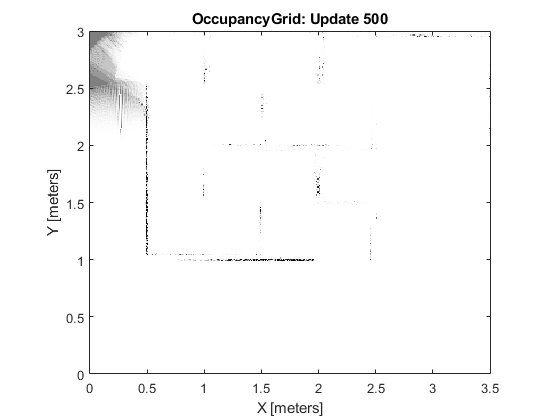
\includegraphics[width=\columnwidth]{./graphics/Prac7_6Occupancy.png}
  	\caption{Occupancy map generated in simulation.}
   	\label{fig:acc1}
\end{figure}
\begin{figure}
   	\captionsetup{width=\columnwidth}
  	\centering
  	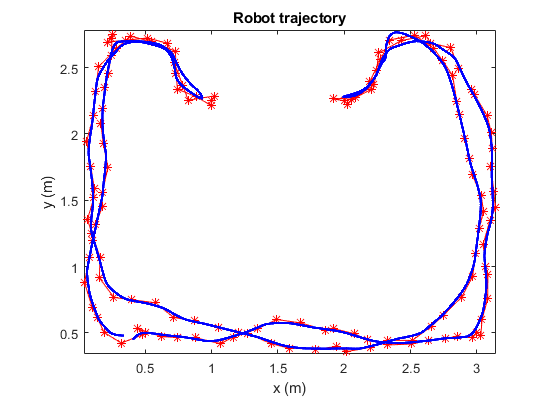
\includegraphics[width=\columnwidth]{./graphics/Prac7_8Trajectory.png}
  	\caption{Simulated robot trajectory from path planning.}
   	\label{fig:tra1}
\end{figure}\begin{figure}
   	\captionsetup{width=\columnwidth}
  	\centering
  	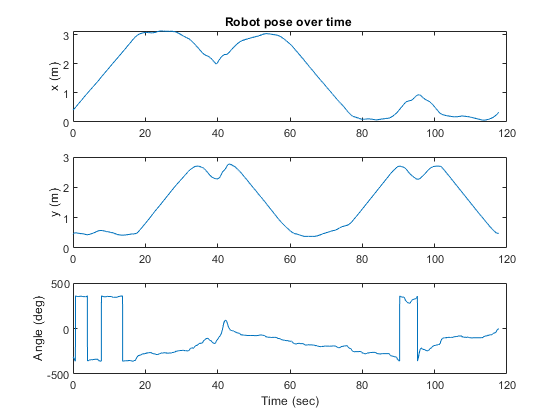
\includegraphics[width=\columnwidth]{./graphics/Prac7_8Pose.png}
  	\caption{Simulated robot pose during figure \ref{fig:tra1} trajectory.}
   	\label{fig:pos1}
\end{figure}

PRM is not a path planning algorithm in and of itself, it simply creates a map of interconnected nodes that can then be used by a path planning algorithm to find a path. The actual path planning algorithm used by the findpath() function is an A* algorithm, which, put simply, tests what would be the shortest possible path from start to finish, a straight line, until an obstacle or the finish is encountered. If the finish has not been encountered it then tests the paths using nodes on either side of the previous path until, once again, an obstacle or the finish is encountered. This process repeats until the finish is actually encountered.\par
\section{Conclusion}
\label{sec:con}

\EOD

\end{document}
